%% BioMed_Central_Tex_Template_v1.06
%%                                      %
%  bmc_article.tex            ver: 1.06 %
%                                       %

%%IMPORTANT: do not delete the first line of this template
%%It must be present to enable the BMC Submission system to
%%recognise this template!!

%%%%%%%%%%%%%%%%%%%%%%%%%%%%%%%%%%%%%%%%%
%%                                     %%
%%  LaTeX template for BioMed Central  %%
%%     journal article submissions     %%
%%                                     %%
%%          <8 June 2012>              %%
%%                                     %%
%%                                     %%
%%%%%%%%%%%%%%%%%%%%%%%%%%%%%%%%%%%%%%%%%


%%%%%%%%%%%%%%%%%%%%%%%%%%%%%%%%%%%%%%%%%%%%%%%%%%%%%%%%%%%%%%%%%%%%%
%%                                                                 %%
%% For instructions on how to fill out this Tex template           %%
%% document please refer to Readme.html and the instructions for   %%
%% authors page on the biomed central website                      %%
%% http://www.biomedcentral.com/info/authors/                      %%
%%                                                                 %%
%% Please do not use \input{...} to include other tex files.       %%
%% Submit your LaTeX manuscript as one .tex document.              %%
%%                                                                 %%
%% All additional figures and files should be attached             %%
%% separately and not embedded in the \TeX\ document itself.       %%
%%                                                                 %%
%% BioMed Central currently use the MikTex distribution of         %%
%% TeX for Windows) of TeX and LaTeX.  This is available from      %%
%% http://www.miktex.org                                           %%
%%                                                                 %%
%%%%%%%%%%%%%%%%%%%%%%%%%%%%%%%%%%%%%%%%%%%%%%%%%%%%%%%%%%%%%%%%%%%%%

%%% additional documentclass options:
%  [doublespacing]
%  [linenumbers]   - put the line numbers on margins

%%% loading packages, author definitions

%\documentclass[twocolumn]{bmcart}% uncomment this for twocolumn layout and comment line below
\documentclass{bmcart}

%%% Load packages
%\usepackage{amsthm,amsmath}
%\RequirePackage{natbib}
%\RequirePackage[authoryear]{natbib}% uncomment this for author-year bibliography
%\RequirePackage{hyperref}
\usepackage[utf8]{inputenc} %unicode support
\usepackage{color}
% \usepackage[applemac]{inputenc} %applemac support if unicode package fails
%\usepackage[latin1]{inputenc} %UNIX support if unicode package fails


%%%%%%%%%%%%%%%%%%%%%%%%%%%%%%%%%%%%%%%%%%%%%%%%%
%%                                             %%
%%  If you wish to display your graphics for   %%
%%  your own use using includegraphic or       %%
%%  includegraphics, then comment out the      %%
%%  following two lines of code.               %%
%%  NB: These line *must* be included when     %%
%%  submitting to BMC.                         %%
%%  All figure files must be submitted as      %%
%%  separate graphics through the BMC          %%
%%  submission process, not included in the    %%
%%  submitted article.                         %%
%%                                             %%
%%%%%%%%%%%%%%%%%%%%%%%%%%%%%%%%%%%%%%%%%%%%%%%%%


\def\includegraphic{}
\def\includegraphics{}



%%% Put your definitions there:
\startlocaldefs
\endlocaldefs


%%% Begin ...
\begin{document}

%%% Start of article front matter
\begin{frontmatter}

\begin{fmbox}
\dochead{Research}

%%%%%%%%%%%%%%%%%%%%%%%%%%%%%%%%%%%%%%%%%%%%%%
%%                                          %%
%% Enter the title of your article here     %%
%%                                          %%
%%%%%%%%%%%%%%%%%%%%%%%%%%%%%%%%%%%%%%%%%%%%%%

\title{A game-theory modeling approach to utility and strength of interactions dynamics in biomedical research social networks}

%%%%%%%%%%%%%%%%%%%%%%%%%%%%%%%%%%%%%%%%%%%%%%
%%                                          %%
%% Enter the authors here                   %%
%%                                          %%
%% Specify information, if available,       %%
%% in the form:                             %%
%%   <key>={<id1>,<id2>}                    %%
%%   <key>=                                 %%
%% Comment or delete the keys which are     %%
%% not used. Repeat \author command as much %%
%% as required.                             %%
%%                                          %%
%%%%%%%%%%%%%%%%%%%%%%%%%%%%%%%%%%%%%%%%%%%%%%

\author[
   addressref={aff1,aff2},                   % id's of addresses, e.g. {aff1,aff2}
   corref={aff1},                       % id of corresponding address, if any
   noteref={n1},                        % id's of article notes, if any
   email={jmario.siqueiros@iimas.unam.mx}   % email address
]{\inits{JMSG}\fnm{J. Mario} \snm{Siqueiros-Garc\'ia}}
\author[
   addressref={aff2},
   email={rgarcia@ie.unam.mx}
]{\inits{RGH}\fnm{Rodrigo} \snm{Garc\'ia-Herrera}}
\author[
   addressref={aff3},
   email={ehernandez@inmegen.mx}
]{\inits{EHL}\fnm{Enrique} \snm{Hern\'andez-Lemus}}
\author[
   addressref={aff3},
   email={sergio.alcala@ciencias.unam.mx}
]{\inits{SAC}\fnm{Sergio} \snm{Alcal\'a-Corona}}



%%%%%%%%%%%%%%%%%%%%%%%%%%%%%%%%%%%%%%%%%%%%%%
%%                                          %%
%% Enter the authors' addresses here        %%
%%                                          %%
%% Repeat \address commands as much as      %%
%% required.                                %%
%%                                          %%
%%%%%%%%%%%%%%%%%%%%%%%%%%%%%%%%%%%%%%%%%%%%%%

\address[id=aff1]{%                           % unique id
  \orgname{IIMAS, Universidad Nacional Aut\'onoma de M\'exico}, % university, etc
  \street{Circuito Escolar 3000, Cd. Universitaria},                     %
  \postcode{04510}                                % post or zip code
  \city{Mexico City},                              % city
  \cny{Mexico}                                    % country
}
\address[id=aff2]{%
  \orgname{LANCIS-IE, Universidad Nacional Aut\'onoma de M\'exico},
  \street{Ciudad Universitaria},
  \postcode{04510}
  \city{Mexico City},
  \cny{Mexico}
}
\address[id=aff3]{%
  \orgname{Instituto Nacional de Medicina Gen\'omica},
  \street{Periferico Sur 4809},
  \postcode{14610}
  \city{Mexico City},
  \cny{Mexico}
}

%%%%%%%%%%%%%%%%%%%%%%%%%%%%%%%%%%%%%%%%%%%%%%
%%                                          %%
%% Enter short notes here                   %%
%%                                          %%
%% Short notes will be after addresses      %%
%% on first page.                           %%
%%                                          %%
%%%%%%%%%%%%%%%%%%%%%%%%%%%%%%%%%%%%%%%%%%%%%%

\begin{artnotes}
%\note{Sample of title note}     % note to the article
\note[id=n1]{Equal contributor} % note, connected to author
\end{artnotes}

\end{fmbox}% comment this for two column layout

%%%%%%%%%%%%%%%%%%%%%%%%%%%%%%%%%%%%%%%%%%%%%%
%%                                          %%
%% The Abstract begins here                 %%
%%                                          %%
%% Please refer to the Instructions for     %%
%% authors on http://www.biomedcentral.com  %%
%% and include the section headings         %%
%% accordingly for your article type.       %%
%%                                          %%
%%%%%%%%%%%%%%%%%%%%%%%%%%%%%%%%%%%%%%%%%%%%%%

\begin{abstractbox}

\begin{abstract} % abstract
%\parttitle{First part title} %if any
Collaboration has become a cornerstone in biomedical research today.
In contrast to physics which has a long history and experience in
collaborative projects, biology is only recently becoming an evermore
collaborative discipline.
In this article we explore the effect of a collaboration network on the distribution
of players having access to certain amount of resources from other players in the
network and the distribution of the strength of connections among
them. Particularly, we implemented two games played simultaneously:
one for maximazing individual utility based on the iterated Prisoner's
Dilemma; the other, a coordination game for maximazing the connection strength
between players. We are interested in how they affect each other in 
the context of a network of scientific collaboration under the idea that while
researchers are interested in maximazing their utilities, they also know that
it is important to invest in building collaborative relationships.
We tested our simulation on a biomedical research community network of M\'exico and
compared the results with an Erd\"{o}s-Reny\'i, a Watts-Strogatz
small-world and Barab\'asi-Albert topologies. Different topologies
display different global utility and global strength of interaction
distributions. Moreover, the distribution of utility and strength of interaction
in the researchers network is similar to that of 
Barab\'asi-Albert and Watts-Strogatz topologies, respectively. We
believe that utility distribution in the researchers network
suggests that there are socio-cultural mechanisms governing the
network that produce an asymmetric distribution of resources. The
high distribution of strong connections might reflect some sort of
subordination among researchers by which they are morally obliged to
cooperate by the same socio-cultural mechanisms. Finally, the range around
the threshold that regulates the decision to cooperate or defect
according to the agent's historical balance between utility and
strength of collaborative relationships and carrying capacity of the
system is small, suggesting that there is a region in which a phase
transition takes place from a population of cooperators to a
population of defectors. Simulations like ours may help to develop
science policies to promote fair distribution of resources.

%\parttitle{Second part title} %if any
\end{abstract}

%%%%%%%%%%%%%%%%%%%%%%%%%%%%%%%%%%%%%%%%%%%%%%
%%                                          %%
%% The keywords begin here                  %%
%%                                          %%
%% Put each keyword in separate \kwd{}.     %%
%%                                          %%
%%%%%%%%%%%%%%%%%%%%%%%%%%%%%%%%%%%%%%%%%%%%%%

\begin{keyword}
\kwd{Collaboration networks}
\kwd{Social Networks Analysis}
\kwd{Biomedicine}
\kwd{Game theory}
\end{keyword}

% MSC classifications codes, if any
%\begin{keyword}[class=AMS]
%\kwd[Primary ]{}
%\kwd{}
%\kwd[; secondary ]{}
%\end{keyword}

\end{abstractbox}
%
%\end{fmbox}% uncomment this for twcolumn layout

\end{frontmatter}

%%%%%%%%%%%%%%%%%%%%%%%%%%%%%%%%%%%%%%%%%%%%%%
%%                                          %%
%% The Main Body begins here                %%
%%                                          %%
%% Please refer to the instructions for     %%
%% authors on:                              %%
%% http://www.biomedcentral.com/info/authors%%
%% and include the section headings         %%
%% accordingly for your article type.       %%
%%                                          %%
%% See the Results and Discussion section   %%
%% for details on how to create sub-sections%%
%%                                          %%
%% use \cite{...} to cite references        %%
%%  \cite{koon} and                         %%
%%  \cite{oreg,khar,zvai,xjon,schn,pond}    %%
%%  \nocite{smith,marg,hunn,advi,koha,mouse}%%
%%                                          %%
%%%%%%%%%%%%%%%%%%%%%%%%%%%%%%%%%%%%%%%%%%%%%%

%%%%%%%%%%%%%%%%%%%%%%%%% start of article main body
% <put your article body there>

%%%%%%%%%%%%%%%%
%% Background %%
%%

\section*{Introduction}

Collaboration has become a cornerstone in biomedical research today.
In contrast to physics which has a long history and experience in
collaborative projects, biology is only recently becoming an evermore
collaborative discipline\cite{VermeulenPenders:2013}. Biology has an
interesting record in such matters because scientific collaboration
means something different to different branches of biology: molecular
biology has traditionally been a research activity of small
laboratories\cite{KnorrCetina:1999,Strasser:2006}, whereas in natural
history there has been data and samples exchange since the $XVII^{th}$
century\cite{MullerWille-etal:2012,Strasser:2012}. Despite the differences in
culture and practices, the Human Genome Project made collaboration a
central feature of biology.\\


Nowadays it is widely acknowledged that collaboration takes many
forms, from sharing of biological samples and biobanking to
international groups in charge of helping research communities to
harmonize and share their data. Sharing resources such as equipment,
funds, and time is critical; building trust among scientists is
fundamental. Also, resources are mobilized in order to create strategic alliances.\\


The analysis of cooperation in scientific research has been the subject of a
number of studies
\cite{VermeulenPenders:2013,Newman:2001,Newman:2004,Elango-etal:2012,HernandezLemus:2013,Strasser:2006,Strasser:2012}. This
is not surprising since cooperation and competition are quite important in
today's academic success. How does collaboration happen within a competitive
academic environment and what kind of payoff is present in these settings were
questions considered recently by Wardil and Hauert \cite{Wardil-etal:2015} in the
context of cooperation in multi-authored publications. Also, the role of game
theory over complex scientific information and collaboration networks has
attracted attention, mainly focusing on how long-term strategies may shape
different scenarios for Nash equilibria \cite{Hanauske-etal:2012}. Prisoner's Dilemma
has been used in the study of impact factor and collaboration
\cite{Hara-etal:2003,LiebermanNowak:2005}. \\  

Even with all these research efforts, cooperation in the context of
scientific collaboration is still loosely defined and the long term
dynamics of academic cooperation (and its consequences) are yet to be
fully elucidated. Furthermore, to our current knowledge, there has
been no use of game theory and complex network analysis for
understanding how the topology of scientific collaboration networks
affects access to resources among individuals present in the network
\footnote{For an account of scientific collaboration and definitions,
  please refer to \cite{Sonnenwald:2007}.}. Our work aims to contribute
to our current understanding on the matter, specially when agents have
to maximize their access to resources while taking care of their collaboration links.\\
  

 In this article we explore the network effect on the distribution
   of players having access to certain amount of resources shared by other players in the
   network and the distribution of the strength of interactions among
   them. Particularly, we implemented two games played simultaneously: 
   one for maximazing individual utility based on the iterated Prisoner's
   Dilemma; the other, a coordination game for maximazing the connection strength between
   players. We are interested in how they affect each other in 
   the context of a network of scientific collaboration under the idea that while
   researchers are interested in maximazing their utilities, they also know that
   it is important to invest in building collaborative relationships. These two
   behaviors are explored in a biomedical research community of M\'exico.\\

In the context of our model, utility represents
  access to resources shared by others.
  The value of the utility function for a player is the sum of the payoffs of playing
  with its neighbors. The opossing force comes from the other concurrent game: players
  trying to maximize the strength of their interactions with other players. In the coordinating game
  the best strategy is to adopt the same strategy as the other player, as it pays the most,
  regardless of cooperation or defection in the utility game. When
  both cooperate the interaction gets a positive payoff, when both defect, the
  interaction doesn't get affected; but if they anti-coordinate, then the
  interaction looses. Finally, cooperation is a central feature of scientific work.
  For our biomedical network, cooperation can be thought of
  as sharing resources such as time, students, equipment, even money. Examples of defection
  to a cooperator are ghost authorship or
  prestige authorship.\\



The manuscript is structured in four sections. First we describe
\textit{FOSISS}, the main program for grants destined to biomedical applied
research in M\'exico. This is the source of the
database from which we created the researchers collaboration network. Next we
describe our model
and the different network topologies on which we explored it.
We then present our results and discuss them. In the last section
we draw some final remarks and conclusions.

\section*{Biomedical research: CONACyT and FOSISS}

CONACyT (National Council of Science and Technology) is the Mexican government
entity in charge of promoting the development of science and 
technology.
Among CONACyT's functions are to develop science and technology
policies according to national needs and demands, to advise the different
instances of government on scientific and technological topics, to promote the
creation of research networks among the scientific community, to grant
scholarships for masters and doctoral studies, and to manage different trusts 
intended to fund individuals and groups for scientific and
technological research.\\

In the year 2002 CONACyT, along with other government agencies and
entities, created sectoral funds
to cover and equally
promote research capacities of different areas such as energy, agriculture
and health. Technological innovation is fostered by the generation of human resources
and by helping research groups to consolidate. It is expected that the
knowledge generated under the sponsorship of these funds
will be the product of applied research that attends national public
needs, and promotes economic growth.\\

\emph{FOSISS} or Sectoral Fund for Health and Social Security Research
(\emph{Fondo Sectorial en Investigaci\'on en Salud y Seguridad Social}) is one of
such funds. FOSISS is constituted by CONACyT, SSA, IMSS and ISSSTE,\footnote{SSA
  is the acronym for Secretariat of Health \emph{Secretar\'ia de Salud}; IMSS is
  the acronym for Social Security Mexican Institute (\emph{Instituto Mexicano
    del Seguro Social}); ISSSTE stands for Institute for Social Security and
  Services for State Workers (\emph{Instituto de Seguridad y Servicios Sociales
    de los Trabajadores del Estado})} all of them being the major public health
providers and research institutions in the country. Every year CONACyT opens a
call for funds limited to a set of health research areas previously defined by a
group of experts. Most applicants are public universities and research
institutions, but eligibility is open to public and private health research sectors.
From 2002 through 2013, there were 91 institutions funded that
comprised 4988 researchers.\\ 

From these data some important considerations should be made
clear. Scientists in the database take on the roles of principal
investigators (PIs), associate researchers, postdoctoral associates,
postgraduate and undergraduate students.
Unfortunately, information on these roles is not specified in the database.
We acknowledge the importance of this deficiency because
researchers in our network act under different circumstances and we know
that this diversity has a real impact on the structure and eventually on the
dynamics of the network, as well as on the results of our model.\\  

Our database includes the
name of the project, the year it was approved for funding and the research area
to which it was assigned. It specifies the names of PIs or the people 
responsible for the project and the names of collaborators.
Researchers can be PIs in one project and collaborators on a different project. The institutional
affiliation of all participants is included. Through this affiliation
we determine the principal institution
behind every project.\\ 

Even though curation and analysis work of this database is still going on, some
relevant facts about the biomedical research can be said. Over the period of 12
years, 32 general research areas have been defined, the three most funded
research areas are \emph{chronic and degenerative diseases}, \emph{malignant
  neoplasms}, and \emph{infectious and parasitic diseases}. The least funded
area is \emph{Ethics and medicine}. The area with the most researchers is
\emph{malignant neoplasms}. Other areas of relevance for M\'exico are
\emph{diseases related to poverty} and \emph{Health and vulnerable groups}. \\  

From the institutions that have participated in a protocol funded by FOSISS,
less than one fifth have been responsible for a project and more than 95\% of
them are Mexican, public institutions. There is also an important presence of
foreign institutions as collaborators, most of them from the United States,
though institutions from the UK, France, Spain, Netherlands, Colombia and Cuba
are also in the database.\\ 

Besides the characteristics of the population there are some other boundary
conditions that play an important role on the network topology and dynamics,
that motivated the development of our model. Biomedical research in M\'exico
constitutes a vibrant community and collaboration is part of everyday
work. However, M\'exico does not have public biobanks for research purposes
(which are specially relevant for research in genomics, for example), there is
no regulation on the access to biological samples such as tissue, cells, DNA,
RNA, etc.\footnote{Regulation exists regarding researcher-subject relations
  based on legal and ethical grounds. Also, all projects need to be approved by
  the Ethics Committee and IRB.} Something similar happens with data. There have
been some attempts to create open data repositories for biomedical research, but
they have not been established yet. Regulation on these subjects is still
missing. Finally, technologically advanced equipment such as high throughput sequencers
are kept by institutions with the highest research
profiles and sometimes PIs manage them in a self serving way.\\  

From our ethnographic work to date, we have been able to see that
biological samples, data and technology can become instruments for negotiating
collaboration. For example, among people involved in research projects, there
are researchers that do not have direct access to samples, simply because their
parent institution does not offer clinical services. Many of them are non medical
doctors but chemists, biologists, physicists, and mathematicians. There is
another group of researchers that are placed on hospitals which is able to do
research and have access to biological samples from their own patients. It seems
that this group is the most privileged one, and the one with the least pressure to establish
collaboration at whatever cost. Finally, there is one more group formed by those
who work as clinicians at small hospitals with no research infrastructure
whatsoever. This group may have an interest in research and the way for them to
become part of a project and be listed as authors in scientific papers is by
giving researchers who do not have access to biological samples access to
patients.\\

Due to these differences in the access to resources, researchers in
general are compelled to build strategic alliances through which samples, data,
technology and authorship, among other assets, become part of a constant flow through
the network. Social and political capital, as well as concentrations of
resources become fundamental tools for establishing fruitful collaborations. 

\section*{Methodology}

%% In this work we developed a model in order to have a better understanding of the
%% distribution of utility and trust in real networks of biomedical research
%% collaboration under certain social constraints  or topological properties.\\  

Our model is based on the iterated version of the Prisoner's Dilemma (PD) and a
coordination game instantiated on
networks. Implementing games on networks is not new and it's an active area of
research aimed to understand the evolution of cooperation in networks populated
by selfish agents \cite{SzaboFath:2007,Nowak-etal:92,OshtukiNowak:2006,Santos-etal:2005,Santos-etal:2006}. In many network models
on which some of game theory games are simulated, agents' decision to cooperate
or defect depend on a specific strategy, such as the well known
\textit{tit-for-tat} \cite{Axelrod:2006,Nowak-etal:2011}. In some other cases, agents
can modify the weight of the interactions with their neighbors
\cite{Santos-etal:2006}. From a different perspective others have explored the effect
of different topologies on the emergence of cooperation
\cite{Santos-etal:2005,HauertDoebeli:2004}. In our model, an agent's decision to
cooperate or defect depends on a balance between
utilities and the current strength of its collaboration relationships. Such
balance reflects the overall success or failure of its strategies. We
study the behavior of the system under different topologies, including a
real-world network.\\  


In our model, agents are embedded in a network with varying number of
neighbors. Following the traditional PD game, the strategy chosen by an agent
and the strategy chosen by its neighbors will produce a pay-off. Pay-off follows
the traditional PD rule: $T > R > P > S$. $T$ is for temptation to defect. It is the highest
pay-off and it takes place when the player defects and the other cooperates. $R$
is for reward for when both players cooperate. $P$ is the punishment for when
both players defect. And $S$ is for suckers pay-off, the worst outcome that
takes place when the player cooperates but its neighbor defects. Utility is a
property of agents in which pay-off is accumulated.\\   

{\bf PD utility pay-off matrix}\\

\begin{tabular}{| l | l | l |}
\hline
          & \bf{Cooperate} & \bf{Defect} \\ \hline
\bf{Cooperate} &  $R,R$      &  $S,T$   \\ \hline
\bf{Defect}    &  $T,S$      &  $P,P$   \\ \hline

\end{tabular}\\ \\

The strength of the interaction, represented by $w$, is a property of the link between two agents and
gets updated according to an $A_{ij}$ matrix of a coordination game. In the $w$ matrix, the highest value
goes to an edge when both agents cooperate, getting an $R$ for reward, if one of
them defects, the connection gets weaker getting $P$ for the collaborative
connection being punished. If both agents defect, the value $w$ doesn't change,
which means that agents didn't interact or that the interaction gets nullified
$N$. In this game, the best action for any agent is to coordinate with its
neighbor, either beacuse it wins or because it doesn't loose. \\ 

{\bf $w$ pay-off matrix}\\

\begin{tabular}{| l | l | l |}
\hline
          & \bf{Cooperate} & \bf{Defect} \\ \hline
\bf{Cooperate} &  $R$      &  $P$   \\ \hline
\bf{Defect}    &  $P$      &  $N$   \\ \hline

\end{tabular}\\ \\


After each game, the agent adds-up utility ($u$), which is the sum of the
pay-offs following the PD matrix. A pair of neighbors will add-up to the strength of
their interaction ($w_{ji}$) as they coordinate or anti-coordinate, being $w$
also cumulative. We measure global utility and connection strength for the whole
network. Global utility $U$ is the sum of all individual utilities and global
strength of connections or $W$ is the sum of every pair of agents' links
$w$. The strength of interaction can be thought as some sort of ``trust''.\\


It should be noted that the same actions or behaviors work for
  both $u$ and $w$. There are two reasons for this decision in the design of the
model. The most general one is that we believe that in the real world,
actions such as cooperating and defecting affect the strength of the interaction
among people. The second one is that we think that selfishly maximizing access to resources and
strengthening relationships are \emph{opposing forces} acting on the same set of
behaviors. The actions of an agent imply a trade-off in which defecting may
increase its utility at the expense of its collaborative relationships. If
collaborators have nourished their relationships, they might be strong enough to
endure occasional defection. Cooperating may build up relationships but it can be
expensive for the player.

\subsection*{Network initialization and agent state update}

All networks are initialized equally. The number of nodes for every network is 4122, the same as in the FOSISS network.
The same utility is given to every agent and all edges are asigned the same weight. In the case of the FOSISS
network, edge weight is given by the number of collaborations among researchers, utility remains the same for all nodes as in
the other networks.\\

The probability for an agent to cooperate or defect depends on a number ($\eta$)
that referes to a historical balance between average utility and the average
strength of the connections with its neigbors. This is so because we assume that
whatever the result in utility or strength of connection, as long as one of them
increases, the player will be confident in the strategy followed so
far. In every simulation step, each player will play both games
  with every neighbor, but set its decision to cooperate or defect beforehand by
  assesing the overall situation of its relationships. This may sound odd, since
  one may think that a person decides for each relationship separately. However
  in this way players are optimizing access to resources and the strength of
  interactions to their neighbors at the same time, since their state is set by
  considering both together.\\  


$\eta$ is calculated as:\\ 


$\eta_i = \frac{\langle f_i \rangle + \langle w_{ij} \rangle _j}{2}$\\

 For the agent to decide whether to cooperate or not, $\eta$ is
  compared to a global threshold $\nu$. If the agents' $\eta$ $>$ $\nu$,
  then the agent will cooperate, otherwise he will be suspicious and will
  defect. $\nu$ is a global parameter that establishes a threshold that an
  agents' $\eta$ must cross in order to decide to cooperate. In this way,
  $\nu$ can limit the size of the population of cooperators. Due
  to what the system and the game can offer to agents in terms of utilities and the strength
  of collaboration relationships, $\nu$ represents the carrying capacity of the
  system for the population of cooperators.\\


Our simulation was tested on an Erd\"{o}s-Reny\'i, a
Watts-Strogatz small-world and Barab\'asi-Albert topologies, as well
as on the real biomedical research collaboration network. The
simulation was run in a synchronous manner, in which all agents update their
behavior simultaneously. \\   

We ran two different experiments. In the first we simulated different
values of carrying capacity $\nu$. With this experiment we were able
to see how the number of cooperators, utility, strength of connections
among agents and the ratio of shifting state population would change
in the range of the carrying capacity. The states of the agents were
the same at initialization, for all values of the carrying
capacity. Since the model is deterministic, it will return the same
result if run under the same conditions.\\

The second experiment consisted in running the simulation under the
same degree of carrying capacity $\nu$ but randomizing the initial
states of the agents. This would show that the system converges to a
global state. For every network, the simulation was run 100 times and
results were averaged.

\section*{Implementation of the model in different topologies}

We built three classical topologies for networks besides the FOSISS network, their parameters are shown in the following table.\\


\begin{tabular}{| l |  l | l |l|l|}
\hline
\bf{Topology}       & $m$              & $\langle k \rangle$          & $\langle C \rangle$      & $\langle l \rangle$ \\ \hline
Erd\"{o}s-R\'enyi  &  $25591$      &  $12.4$        &  $0.003$ & $3.6$  \\ \hline
Watts-Strogatz    &  $206100$   &  $100$         &  $0.7$      & $3.4$  \\ \hline
Barb\'asi-Albert    &  $183465$   &  $89$           &  $0.06$    & $2.13$ \\ \hline
FOSISS                    &  $23391$     &   11.39     &  $0.87$    &  $5.49$ \\ \hline
\end{tabular}\\ 


\subsection*{Erd\"{o}s-Reny\'i}

Erd\"{o}s-Reny\'i networks \cite{ErdosRenyi:59} (random networks) are constructed by randomly selecting a pair of $N$ possible nodes and attaching them with an edge, given a probability $p$, as long as there is no edge between them. The result is a Poisson distribution for connectivity of nodes $P(k)$, where each node has a degree quite close to the average $\langle k \rangle$. Also for this type of network, average clustering coefficient  $\langle C \rangle$ is small, actually it is equal to $p$ (the probability of connecting two nodes) and the average shortest path length $\langle l \rangle = \frac{lnN}{ln\langle k \rangle}$.


\subsection*{Small-World}

Watts-Strogatz networks \cite{WattsStrogatz:98} (small-world networks) are in a regime between a fully regular grid (lattice) and a random network (Erd\"{o}s-R\'enyi). In order to build them, a node is chosen from a lattice (a ring) and the edge that connects it to nearest neighbor in a clockwise sense. With probability $p$, this edge is reconnected to a node chosen uniformly at random over the entire ring, with duplicate edges forbidden; otherwise the edge is left in place. This process is repeated by moving clockwise around the ring, considering each node in turn until one lap is completed. Next, the edges connect nodes to their second-nearest neighbors clockwise. As before, each of these edges is randomly rewired with probability $p$. This process continues, circulating around the ring and proceeding outward to more distant neighbors after each lap, until each edge in the original lattice has been considered once. The main characteristic of these networks is that the average shortest path length is small and grows as $log(N)$ ($\langle l \rangle \sim log(N)$). Also, the average clustering coefficient $\langle C \rangle$ remains large in terms of $p$. For $p < 0.1$, $\langle C \rangle \sim 1$.

\subsection*{Barb\'asi-Albert}

Barb\'asi-Albert networks \cite{BarabasiAlbert:99} (scale-free networks) are generated by adding new nodes to a network. Each new node is added connecting it to an existing node with a probability proportional to the degree $k$ (connectivity) of each node (\textit{preferential attachment}). The result is a a power law distribution for connectivity of nodes $P(k)$ where few nodes have many connections and the most have very few connections. Furthermore these networks are also small world networks, showing a quite small $\langle l \rangle$.


\subsection*{FOSISS: Biomedical research community network}

The biomedical research network on which we are running our model was generated 
with data from collaborative projects. Our data was obtained from CONACyT and includes information for twelve years of \textit{FOSISS} grants. Data included names of Principal Investigators, collaborators, research topics, etc. The network we are using here has researchers as nodes and edges represent the connection of two scientists when they colaborate on the same project. Edges are also weighted according to the number of projects shared by any pair of scientists.\\

\section*{Results}

In this section we present the main results of the study, namely the topological
structure of the underlying network models, the dynamics of the games under
different parameters and network topologies and the distribution of utility and
of the strength of interaction resulting of playing the games in all the
different scenarios considered, including the real FOSISS network.\\


FOSISS network summed-up a total of 145 components or subnetworks, but we ran
the model on the giant component made-up of 4122 researchers, and 23391 edges.
The giant component was analyzed using \textit{Cytoscape} \textbf{Figure
  1}. Results show that it is a well integrated network, with a clustering
coefficient $\langle C \rangle = 0.870$, an average shortest path length of
$\langle l \rangle = 5.493$  and a density of $p = 0.003$. Such properties
recall a small-world topology \cite{WattsStrogatz:98}, and a great deal of
self-organization when compared to a random network with the same density and
number of nodes. Network centralization is $0.023$, since there are no visible
researchers that play as hubs in the network. Nevertheless the network
heterogeneity is $0.873$, which means that the network is highly
hierarchical. When the degree distribution is analyzed, degree decreases as a
power-law with an exponent of $1.7$, similar to other social networks described
as scale-free topology networks \cite{BarabasiAlbert:99}. Finally, the average number
of neighbors of each node is $11.39$ \cite{Shannon:2003}.\\


\begin{figure} [h!]
\centering
% 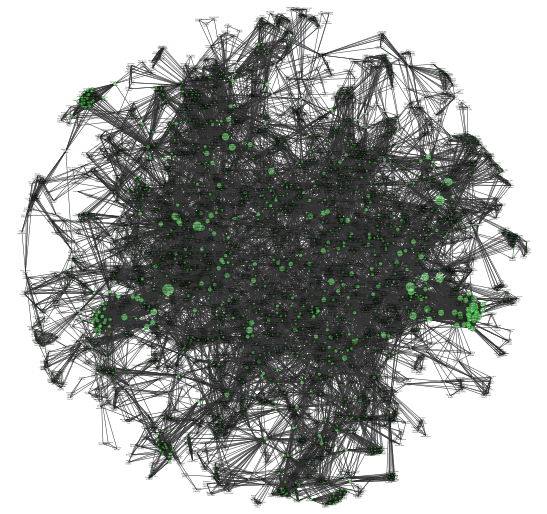
\includegraphics[scale=0.5]{images/Fosiss_GC_final.png}
\caption{Bioemdical research collaboration network (FOSISS) giant component.}\label{Fosiss_GC}
\end{figure}

%\FloatBarrier

Other results to report are those of the dynamics of different
variables as the carrying capacity $\nu$ changes. The  most salient
result is that for $\nu$ between $0.19$ and $0.24$, there is an
apparent phase transition in all different topologies and for all the
different variables. It is worth noting that the shape
of the phase transition-like behavior is different according to the topology of the
network under study. When $\nu$ is between $0.0$ and $0.2$, that is, when there is
no space or a very short one for suspiciousness, all agents cooperate, when
$\nu$ is above $0.25$, all agents defect. \textit{Utility},
\textit{strength of interactions}, and \textit{changing state population}
replicate that same behavior for the same limits. \\ 

In \textbf{Figure 2}, we present how the number of cooperators in the population
change as $\nu$ changes. In the Erd\"{o}s-Reny\'i, network, between $0$ and
$0.18$ approximately, all agents converge to a cooperative behavior, from $18$
to $20$, convergence to cooperative state takes longer but eventually all agents
are cooperating. Close to $\nu \approx 0.21$ there is a sharp fall to a point in
which around half the population is cooperating and the rest is
defecting. Reaching $\nu \approx 0.25$ there is another sharp fall of
cooperators and all agents turn into a defecting state.\\


In the case of the Watts-Strogatz, small-world network, the whole
population remains cooperating for ranges between $0$ and $0.2$ but as
it gets closer to $0.2$, more time is needed for the population to
become full of cooperators. In $\nu \approx 0.2$ the cooperators will
represent only half of the population and such number of them will be
constant up to $\nu \approx 0.25$ forming a short plateau. From $\nu
\approx 0.25$ to $\nu \approx 0.6$ cooperators will be present at the
beginning of the simulation but will diminish as time goes on.  In the
case of the Barab\'asi-Albert network, crossing the threshold of $\nu
\approx 0.2$, there is a sharp decrease in the number of cooperators,
but stays constant over time. Such behavior is present for a very
short range of $\nu$, and before $\nu \approx 0.24$, cooperators
disappear for the rest of values of $\nu$. Finally, FOSISS network
behaves similarly to the other networks in that there is a fall in the
number of cooperators close to $\nu \approx 0.2$. In contrast with the
other networks, the FOSISS network lacks the sharp reduction of
cooperators, instead this population declines smoothly and
progressively; specially, when it reaches a $\nu \approx 0.25$
cooperators decrease in a less dramatic manner all the way to
$\nu \approx 0.5$. It is also noteworthy that from $\nu = 0$ to $\nu
\approx 0.5$ the number of cooperators converge to a certain degree
and stays constant for the rest of the simulation.\\


\begin{figure} [h!]
\centering
\begin{tabular}{cc}
%   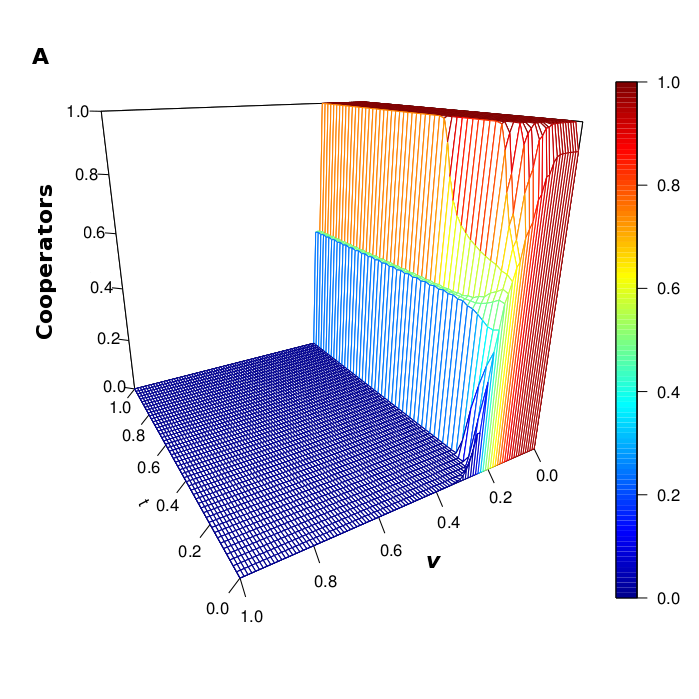
\includegraphics[scale=0.28]{images/erdos_dc_nus_1.png} & 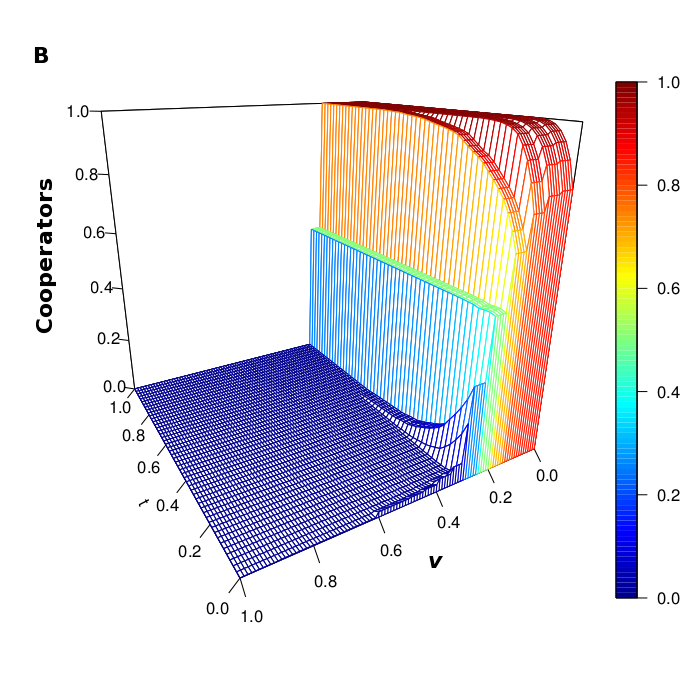
\includegraphics[scale=0.28]{images/watts_dc_nus_1.png}
%   \\
%   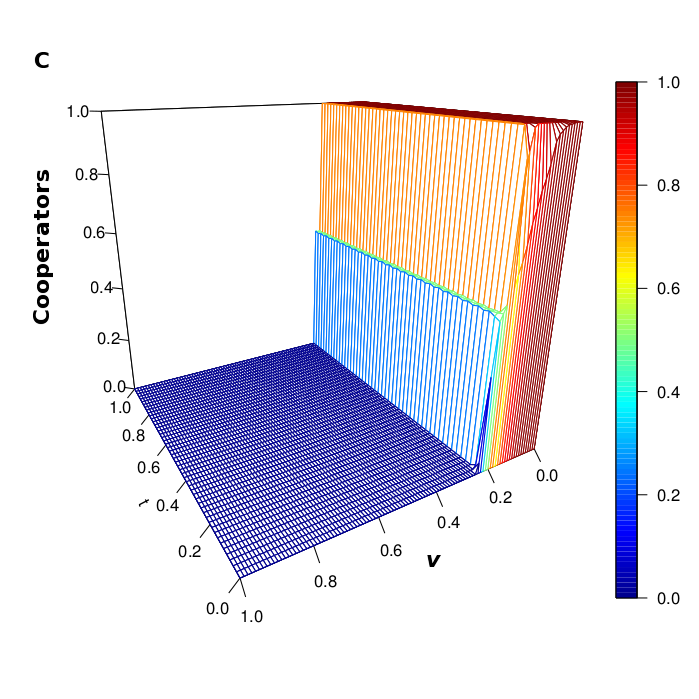
\includegraphics[scale=0.28]{images/barabasi_dc_nus_1.png} & 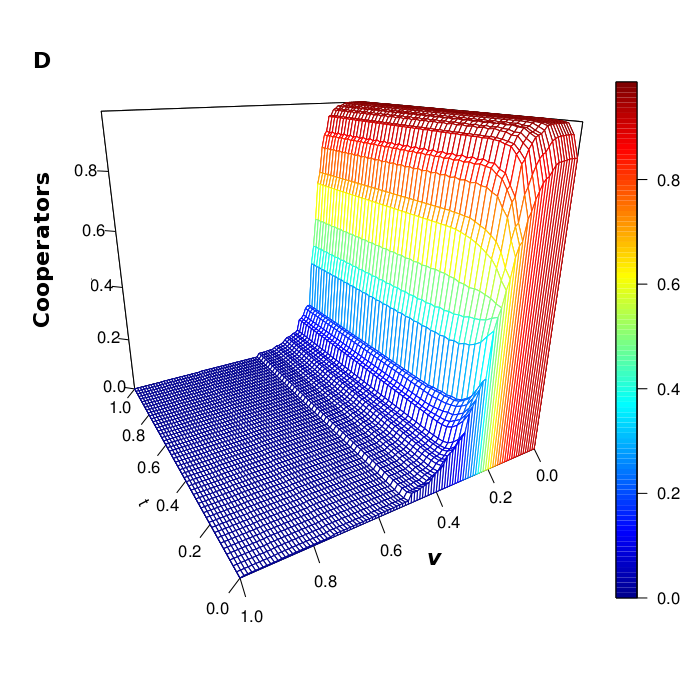
\includegraphics[scale=0.28]{images/fosiss_dc_nus_1.png}
\end{tabular}
\caption{Ratio of cooperators as a function of carrying capacity and time. Topologies are: A. Random, Erd\"{o}s-R\'enyi. B. Watts-Strogatz. C. Barab\'asi-Albert. D. FOSISS.
}\label{CD}
\end{figure}

% \FloatBarrier

Utility and strength of interactions dynamics under different $\nu$ are similar to the
phase transition found before. \textbf{Figures 3 and 4} show
that there is a drop in utility and strength of interactions according to the
drop in the number of cooperators. Erd\"{o}s-Reny\'i and Barab\'asi-Albert
networks are quite similar in the way these variables fall in two steps, the
first one at $\nu \approx 0.2$ and the next one at $\nu \approx 0.23$. The fall
is sharper still in the Barab\'asi-Albert topology. Utility and strength of
interactions phase transition in Watts-Strogatz network is significantly more
staggered compared to the former networks. In the case of utility, there is a
region in the limits of $\nu \approx 0.25$ and $\nu \approx 0.3$, before utility
goes to $0$, in which it remains low but stable over time. In general, strength
of interactions follows the same pattern as utility but in the same $\nu \approx
0.25$ and $\nu \approx 0.3$, strength of interactions grows to a value that is
higher than the one given by default but soon starts to decrease as the
simulation runs. For the FOSISS network, utility and interaction strength fall
quite steeply but smoothly, without sharp cuts. Between $\nu \approx 0.23$ and
$\nu \approx 0.28$, utility and strength of interactions start at their lowest,
but there is a slight increase in both of them.\\


\begin{figure} [h!]
\centering
\begin{tabular}{cc}

% 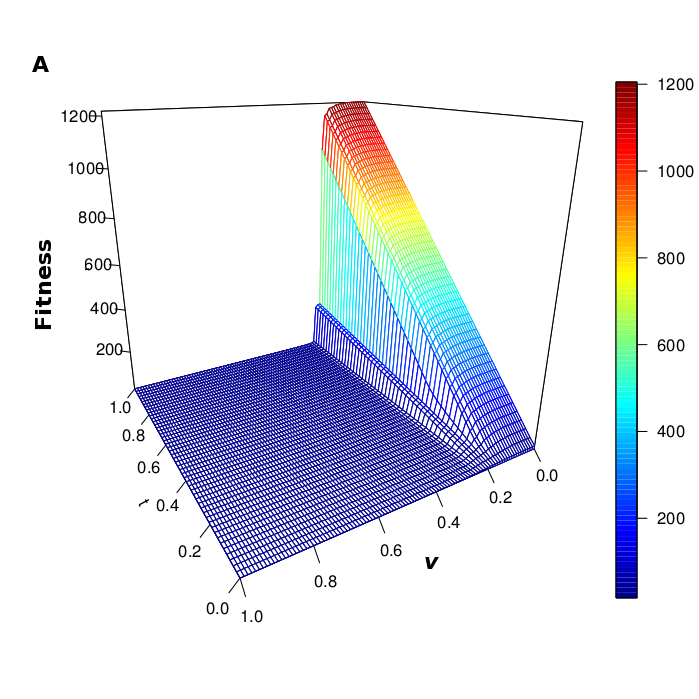
\includegraphics[scale=0.28]{images/erdos_fitness_nus_1.png} & 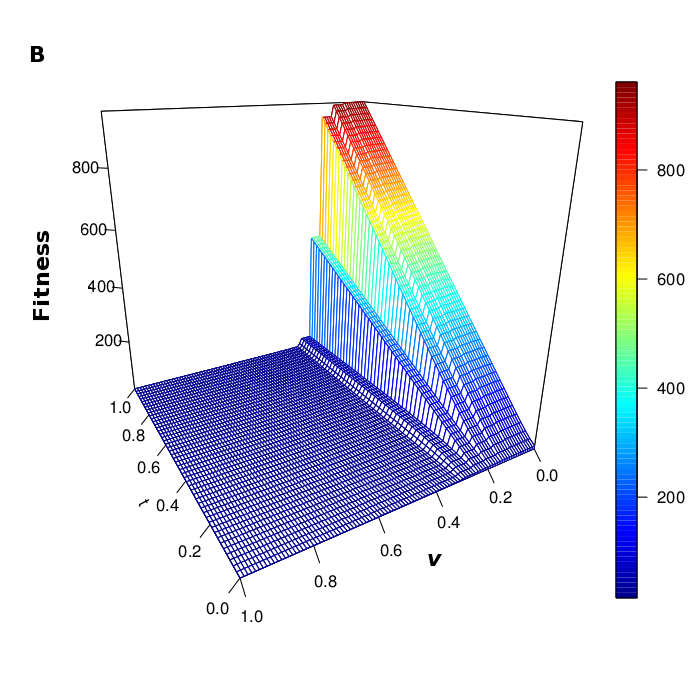
\includegraphics[scale=0.28]{images/watts_fitness_nus_1.png} \\
% 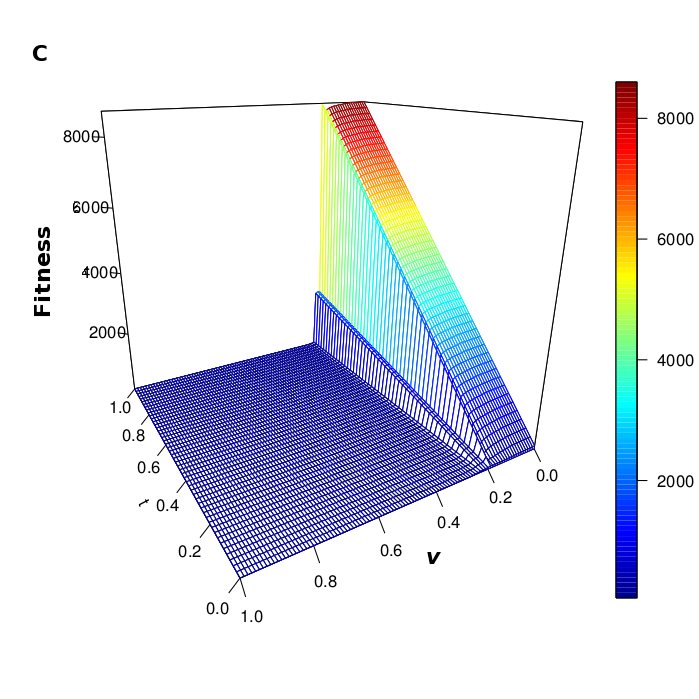
\includegraphics[scale=0.28]{images/barabasi_fitness_nus_1.png} & 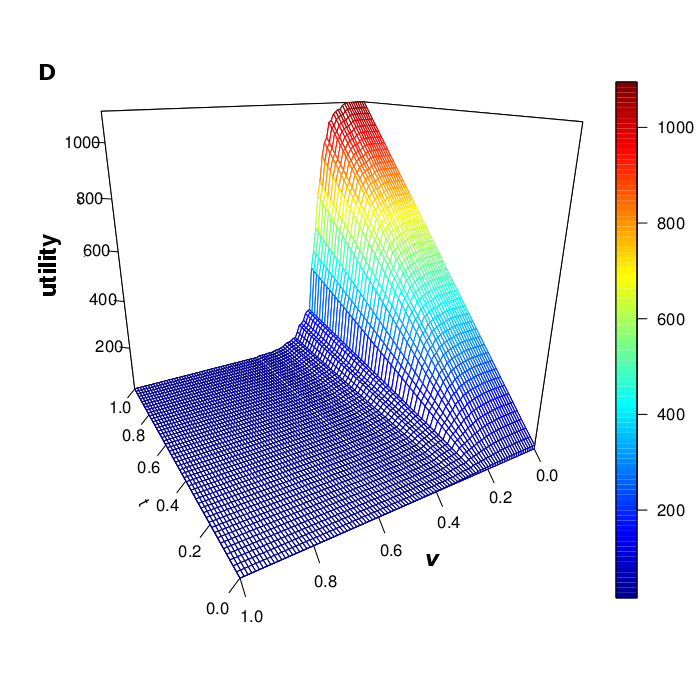
\includegraphics[scale=0.28]{images/fosiss_fitness_nus_1.png}
\end{tabular}
\caption{Utility $U$ dynamics as a function of carrying capacity $\nu$ and time. Topologies are: A. Random, Erd\"{o}s-R\'enyi. B. Watts-Strogatz. C. Barab\'asi-Albert. D. FOSISS.}\label{fitness}
\end{figure}

% \FloatBarrier


\begin{figure} [h!]
\centering
\begin{tabular}{cc}

% 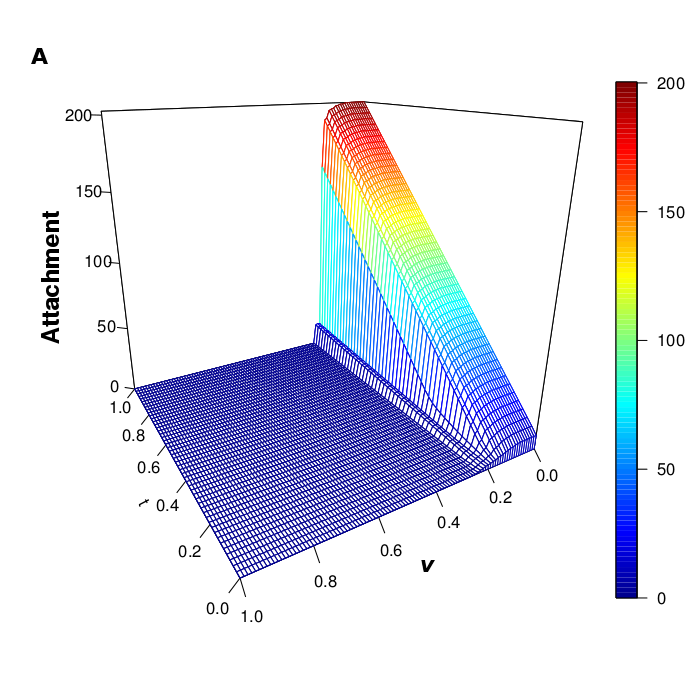
\includegraphics[scale=0.28]{images/erdos_trust_nus_1.png} & 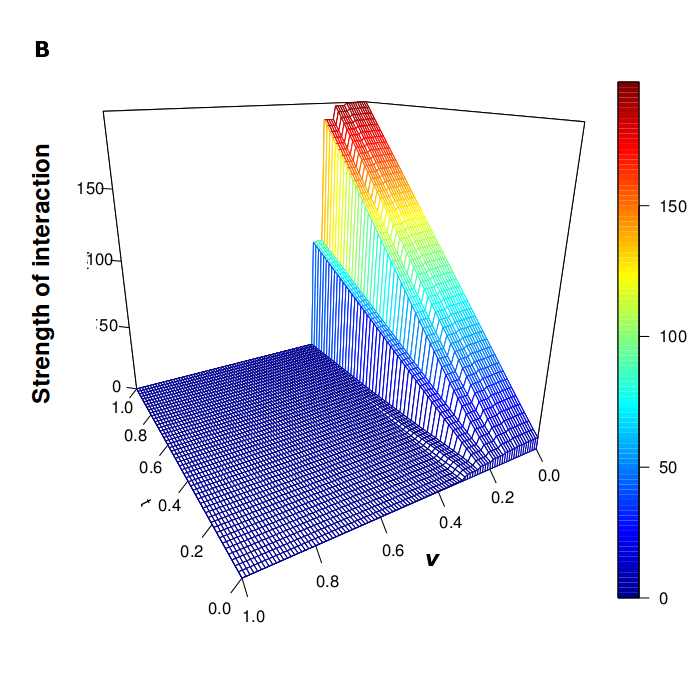
\includegraphics[scale=0.28]{images/watts_trust_nus_1.png} \\
% 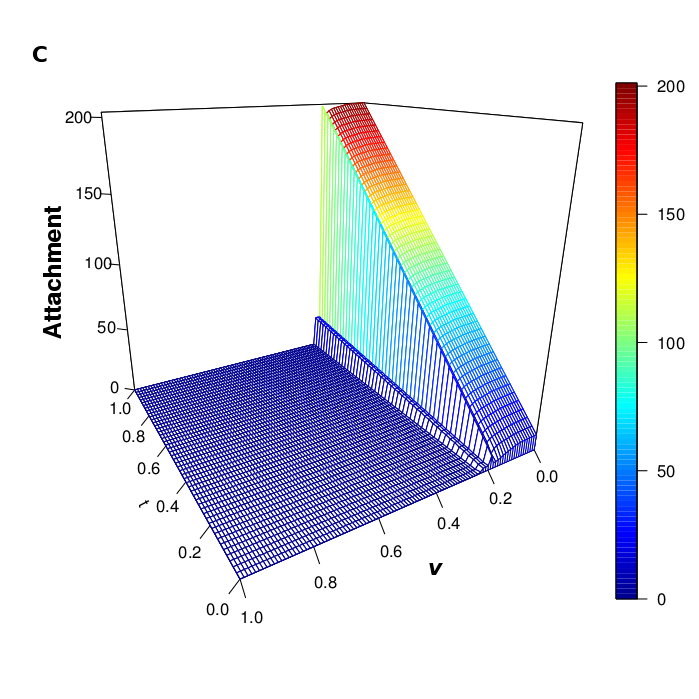
\includegraphics[scale=0.28]{images/barabasi_trust_nus_1.png} & 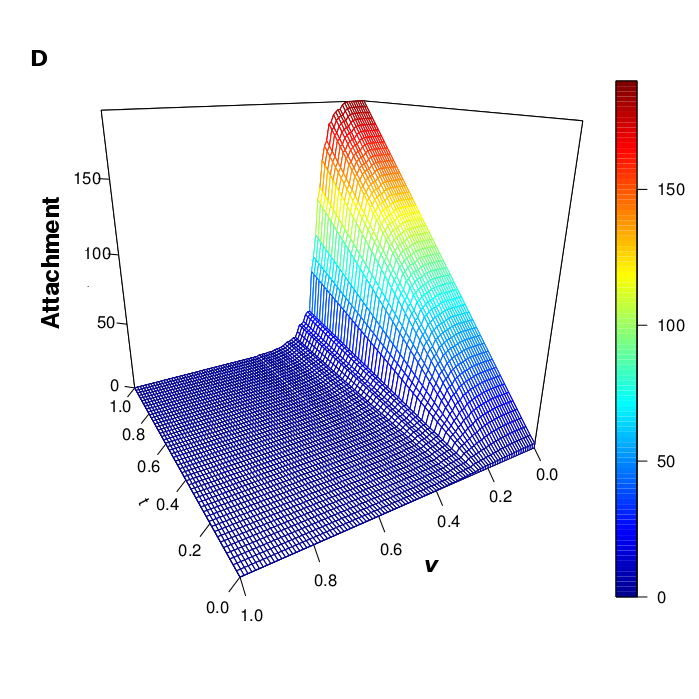
\includegraphics[scale=0.28]{images/fosiss_trust_nus_1.png}
\end{tabular}
\caption{Strength of interactions $w$ dynamics as a function of carrying capacity $\nu$ and time. Topologies are: A. Random, Erd\"{o}s-R\'enyi. B. Watts-Strogatz. C. Barab\'asi-Albert. D. FOSISS.}\label{trust}
\end{figure}

% \FloatBarrier

We also measured the number of agents shifting states --between cooperating and
defecting- under different $\nu$ values. We found that for all networks there is
a critical point around  $\nu \approx 0.2$ in which all agents are shifting
states. For Erd\"{o}s-Reny\'i and Barab\'asi-Albert networks, for this region,
agents never settle to a single state. Contrary to the former cases, the number
of shifting agents decreases considerably for the Watts-Strogatz and FOSISS
networks, and find an equilibrium state. Once the the limits of this region are
crossed as $\nu$ increases, the number of agents shifting states falls to $0$
and all nodes become defectors. \\


\begin{figure} [h!]
\centering
\begin{tabular}{cc}

% 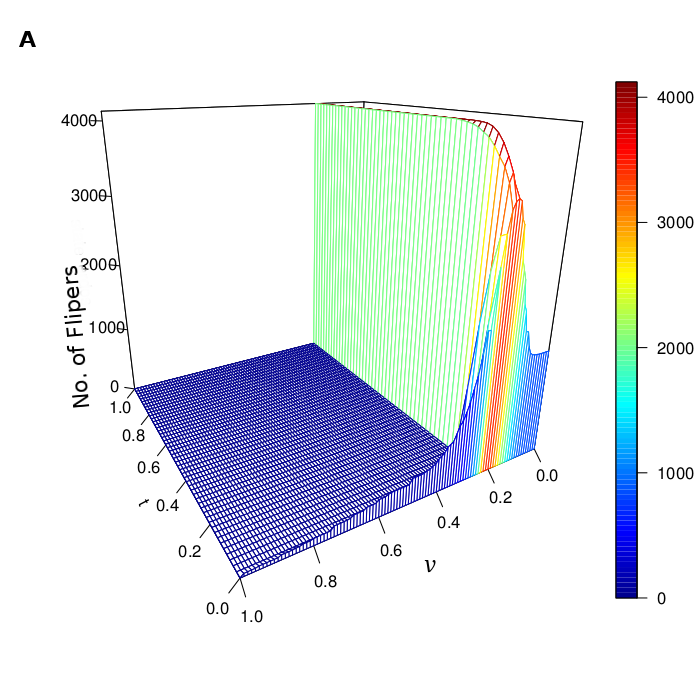
\includegraphics[scale=0.28]{images/erdos_state_nus.png} & 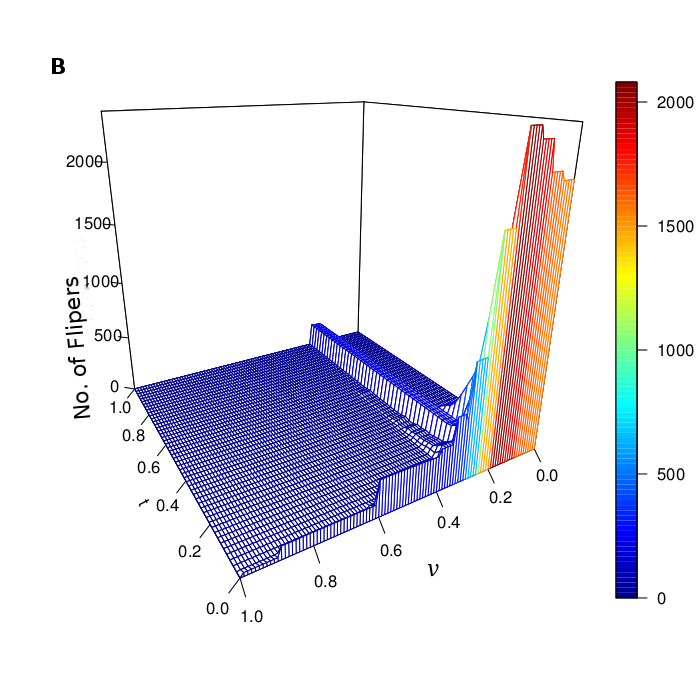
\includegraphics[scale=0.28]{images/watts_state_nus.png} \\
% 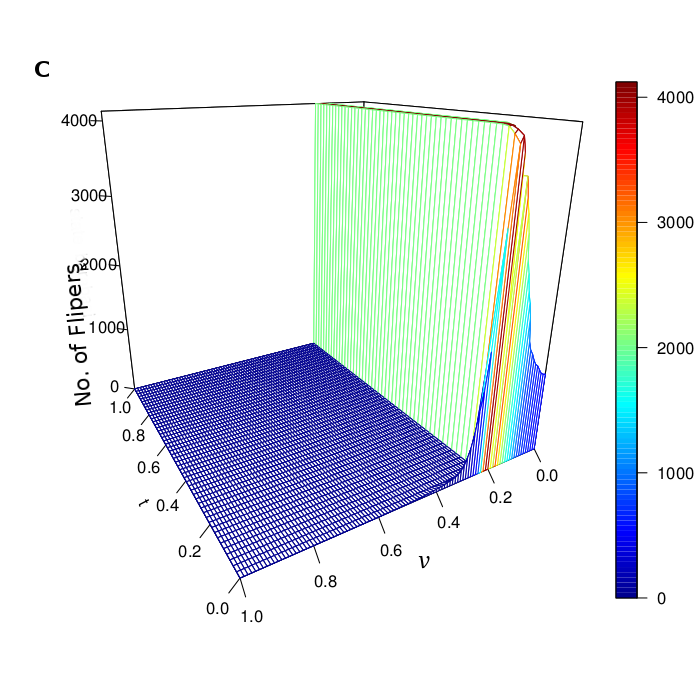
\includegraphics[scale=0.28]{images/barabasi_state_nus.png} & 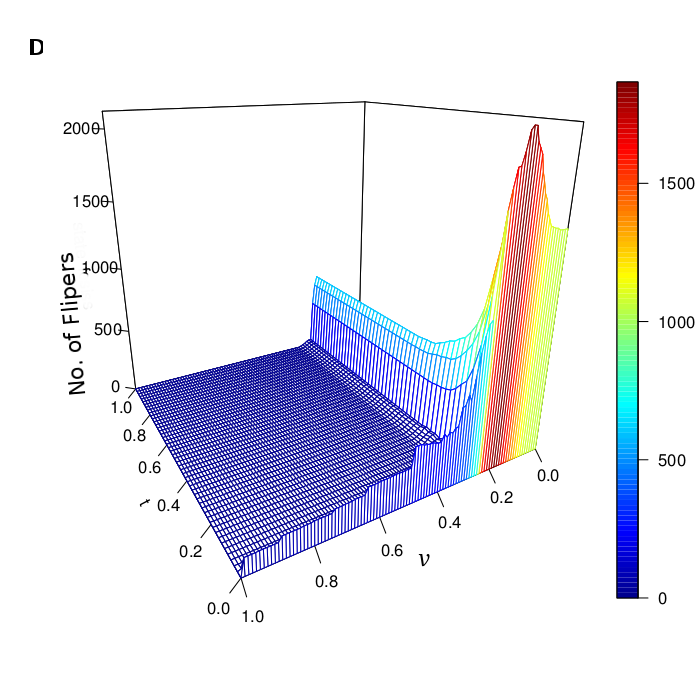
\includegraphics[scale=0.28]{images/fosiss_state_nus.png}
\end{tabular}
\caption{Shifting population between cooperators and defectors as a function of
carrying capacity $\nu$ and time. Topologies are: A. Random, Erd\"{o}s-R\'enyi. B. Watts-Strogatz. C. Barab\'asi-Albert. D. FOSISS.}\label{state} 
\end{figure}

% \FloatBarrier

Central to our argument is the differences in utility and strength of
interactions distribution at the end of the simulation, for every topology. We
found that utility distribution for the \textit{FOSISS} network, resembles quite
accurately to the distribution of utility in the Barab\'asi-Albert
network.\\ 


The distribution of utility on each topology is induced by the degree
distribution. This is so, since a given agent (node) will interact with its
neighbors to either cooperate or defect, in such a way that connectivity
influences the number of events played and thus the likelihood of increasing its
corresponding utility. For instance, utility distribution in the random,
Erd\"{o}s-R\'enyi network displays a normal-like curve. The algorithm that
generates this kind of topology, assigns to every node the same probability of
connecting with any other node, which produces a \textit{poissonian} degree
distribution \cite{ErdosRenyi:59}. Since the Watts-Strogatz degree distribution is
described by a function that is midways between a random distribution and a
scale-free network \cite{Barratmodels:2000} one may expect also  an intermediate
behavior of the utility distribution. This assumption seems to be fulfilled by
the distribution in Figure 6B. \\

The resemblance of the degree-distribution and utility distribution also holds
for the Bar\'abasi-Albert network. As mentioned in the methods section, the
degree distribution of a Bar\'abasi-Albert topology follows a power-law that
describes the fact that there are a small number of nodes with large $k$ and most
nodes have a small $k$ \cite{BarabasiAlbert:99}. As it is shown in the following
figure, most utility is concentrated in a few number of agents, while most
agents have a small amount of it. This is consistent with other research in
which concentration of resources, fame or citations in science decreases as a
power-law \cite{Simon:55,Price:1965,Merton:1968}. FOSISS network utility
distribution is also skewed to the left, similar to that of the
Barab\'asi-Albert network. \\ 


\begin{figure} [h!]
\centering
\begin{tabular}{cc}

% 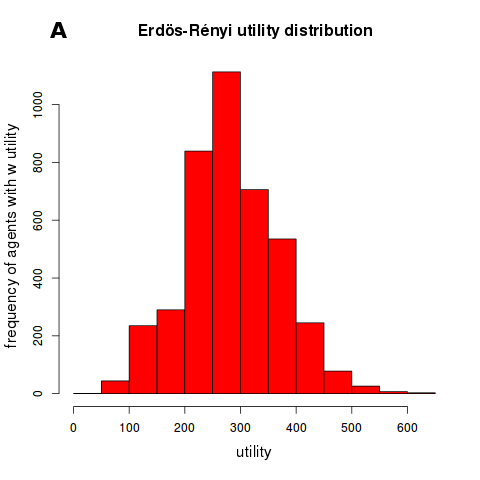
\includegraphics[scale=0.28]{images/erdos_fitness.png} & 
% 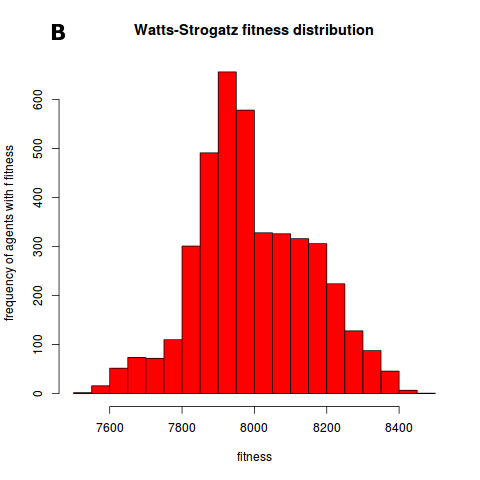
\includegraphics[scale=0.28]{images/watts_fitness.png} \\
% 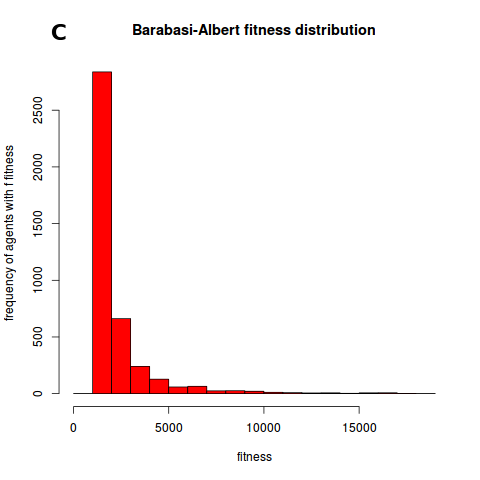
\includegraphics[scale=0.28]{images/barabasi_fitness.png} & 
% 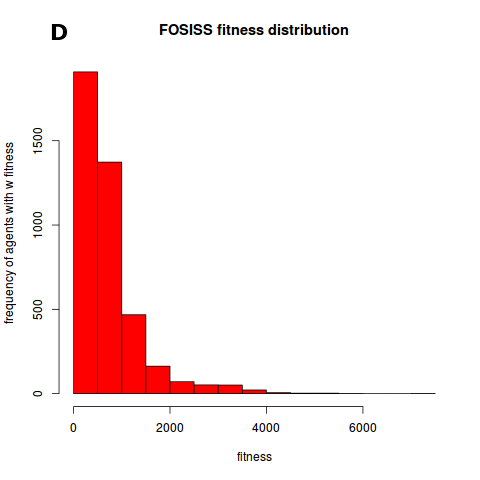
\includegraphics[scale=0.28]{images/fosiss_fitness.png}
\end{tabular}
\caption{Utility distribution on different topologies. A. Random,
  Erd\"{o}s-R\'enyi network displays a normal-like
  distribution. B. Watts-Strogatz network utility distribution is highly skewed
  to the right. C. Barab\'asi-Albert network. Utility is distributed highly
  skewed to the left. D. FOSISS, biomedical researchers collaboration network
  distribution of utility resembles to Barab\'asi-Albert
  network.}\label{histo_fitness} 
\end{figure}

% \FloatBarrier

Regarding strength of interactions distribution, the Erd\"{o}s-R\'enyi random
network displays a normal distribution of strength of interactions, as
expected. Again strength of interactions values are highly influenced by the
corresponding degree distribution (Figure 7A). However, in the Watts-Strogatz
network topology (Figure 7B), the strength of interactions distribution is a
highly asymmetric bimodal, with a really-low frequency mode of low strength of
interactions and a highly probability mode for high strength of interactions. A
possible explanation for this phenomenon is that under network topologies
maximizing inter-node communication (by minimizing the average distance between
nodes) such as the Watts-Strogatz, strength of interactions is favored both
among the cooperators (constituting the majority of players) and the
defectors. \\ 


The Barab\'asi-Albert network (7C) presents also a symmetric unimodal
distribution with values higher (on average) than those of the Erd\"{o}s-R\'enyi
random network, this may be the effect of increased communication due to more
efficient network navigability. Interestingly, the network corresponding to the
real FOSISS collaborations (7D) is an asymmetric unimodal distribution in which
moderate to high values of strength of interactions are more likely. We 
hypothesize that this effect is also due to the communication properties of the
network. \\

\begin{figure} [h!]
\centering
\begin{tabular}{cc}

% 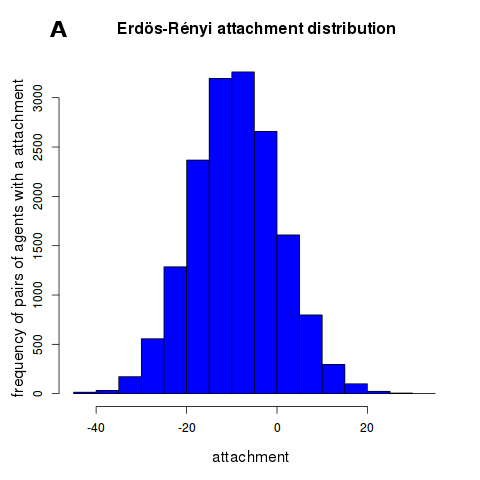
\includegraphics[scale=0.28]{images/erdos_trust.png} & 
% 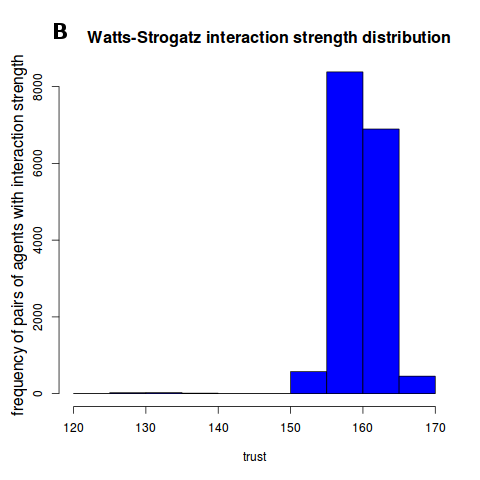
\includegraphics[scale=0.28]{images/watts_trust.png} \\
% 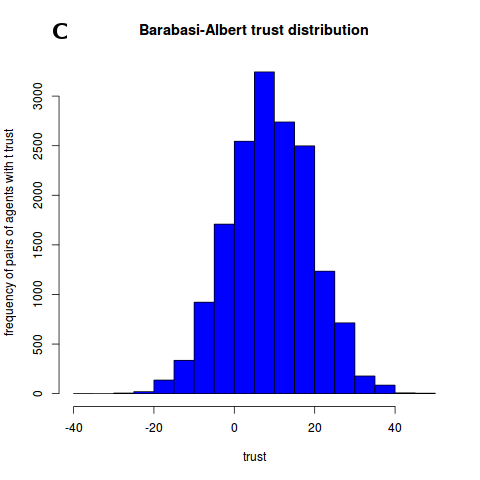
\includegraphics[scale=0.28]{images/barabasi_trust.png} & 
% 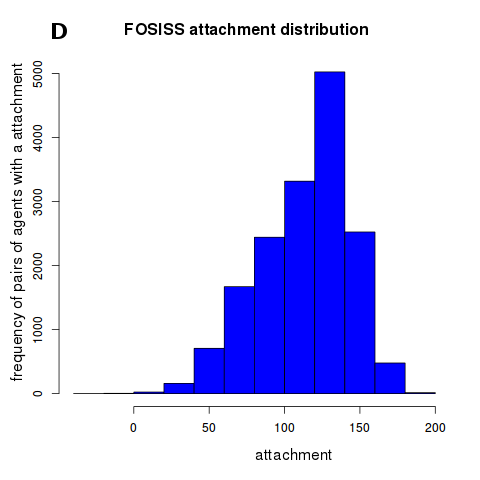
\includegraphics[scale=0.28]{images/fosiss_trust.png}
\end{tabular}
\caption{Strength of interactions distribution on different topologies. A. Random, Erd\"{o}s-R\'enyi network displays a normal-like
distribution. B. Watts-Strogatz network strength of interactions distribution is bimodal and highly skewed to the right. C.
Barab\'asi-Albert network strength of interactions distribution is also a
normal-like curve. D. FOSISS, biomedical researchers collaboration network distribution of strength of interactions is skewed to the right.}\label{histo_trust}  
\end{figure}

% \FloatBarrier

An interesting feature of highly communicated networks (characterized
by high values of clustering coefficient) is the fact that certainty
among players seems to be enhanced, that is, in such networks the rate
of change of strategy is significantly lower (and smoother) than in
poorly connected networks. This is another instance in which easier
communication (i.e. lower average minimum path lengths) leads to better
performance of the whole collaborative research system.\\

\section*{Discussion}
\label{sec:3}

In this work we have analyzed the influence of parameters
  given by the underlying social structure of a science collaborative
  network on collective strength of interactions and utility dynamical
  behavior, based on a class of iterated PD and coordination
  games. Such parameters include mainly local and global connectivity
  like the degree centrality and average clustering coefficient, as
  well as communication patterns.\\

  Under the assumptions given by the model, we were able to
  notice that, in general, communication within the social
  collaborative networks has a positive correlation with average
  strength of interactions between the individuals partaking in the
  games and also with the global collective utility (given by the sum
  of the individual payoffs). The better the communication among
  players, the higher the strength of interactions and the utility
  leading to an optimized functioning of the whole \emph{scientific
    collaboration system}. This is an important result that may be
  useful for scientific policy planning and may set a foundation for
  the optimal use of social networks in scientific collaboration as a
  means to improve the relationships among collaborating peers and
  ultimately the performance of research systems.  We obviously need
  more qualitative work in order to validate these results from a
  sociological and anthropological perspective.\\

%Furthermore, such validation is necessary because, as we said at
%the beginning of this work, \emph{strength of
%interactions} can have many different meanings and
%implementations in the real world. The same we can say
%about \emph{utility} and most of all, about the idea of the game we
%explored here since ``playing the
%game'' must have so, many different meanings among
%resarchers and their communities.\\

  \section*{Conclusions}
  
  
 To close this article, we would like to comment on three
  issues we consider important. The first one is about confronting our
  results with data available to us from the biomedical research
  community. Second, some remarks we believe are important about the
  role of computational simulations in the social sciences. Finally we
  would like to comment on our future work.\\


  The two main results of our model are the smoothness in
  the phase transition-like behavior for different parameters and the
  distribution of utility and strength of interactions in the FOSISS
  network compared to other networks and their topologies. We are
  certain that the particular structure of FOSISS network is playing a
  central role in the results and because of that we would like to
  discuss it a little bit further.\\

  FOSISS network is higly hierarchical according to its
  heterogeneity of $0.873$. Because of it, one would expect to find
  the presence of important hubs \cite{Wu:2008}, that is, a few
  researchers control the whole network, as has been reported in some
  other places \cite{yousefi-etal:2008}. Surprisingly, FOSISS network
  centralization is very low $0.023$, i.e. there are no researchers
  that centralize the majority of connections. Our guess is that the
  network is composed of many small communities or groups with a
  central researcher or Principal Investigator (PI). If this is the
  case in the FOSISS network, it means that those groups have a very
  hierarchic structure as well.\\

  Under such structure, when the clustering coefficient is
  considered, it can be said that groups are also well connected but
  that inter-group connections are sparse. In other words, individual
  groups are strongly connected within but the network as a whole is
  supported by a small number of links. We came by this idea partially
  from another study about scientific collaborations based on
  co-authorships in one of the research centers that is part of the
  FOSISS network \cite{HernandezLemus:2013}. In the cited reference an
  apparently well integrated community was found (high clustering
  coefficient and a very short characteristic path length). Such
  integration was mostly superficial, since it depended on the
  presence of external collaborators from other research institutions
  (most of them from overseas).  Removing these external collaborators
  brakes down the network into small subgraphs that worked
  independently. Remarkably those subgraphs corresponded to the real
  groups of that research center.  What is more, several groups had a
  hierarchical structure as the one we suspect is common in FOSISS
  subgraphs. The results showed that collaboration was poor between
  groups but strong among the members of each group, and that
  collaboration among groups doesn't emerge bottom-up, instead it
  seems to be promoted from the top, from the administrative
  authorities.\\

  We believe that the the situation just refered is also
  true for the whole biomedical research community in M\'exico. The
  amount of PIs who have also been collaborators in other projects is
  about one fifth of the total number of participants.  This is a
  number big enough to connect the whole network in one giant
  component. Yet, due to the topological characteristics of the FOSISS
  network, it appears to be the case that researchers can be the
  leaders in one project and collaborators of different project of
  \emph{its own research group}. CONACyT's funding policies makes it
  impossible for a researcher to get a grant from a fund if that
  researcher has an ongoing project with a grant from that same
  fund. That is, a researcher can ask for a grant from FOSISS if and
  only if at the moment he doesn't already have one.
  This policy has lead researchers from the same group to ask
  for grants from the same fund in order to rise their budgets. A
  consequence of this behavior is that group interactions get
  reinforced, but integroup connections not necessarily so.\\

 As is common among scientific communities in biomedical
  research, PIs play a central role in the network. Strong PIs and
  well connected groups seem to be somehow responsible for the high
  levels of strength of interactions and the centralization of utility
  in our simulation. As for what seems to be phase transitions, in the
  case of FOSISS networks, these are smoother than those in the other
  networks with different topologies, even for those with a
  small-world topology. We think that this behavior is also the result
  of the hierarchical structure already mentioned. If this is true,
  strength of interactions is first lost in the edges that link
  diffrent goups and then in the edges that connect members of the
  groups. Connections between groups would not be as dense as those
  inside the groups, which means that there would not be enough
  information of the behavior of one group regarding its neighbors to
  constrain them as it seems to happen with individual researchers
  inside their communities. Nevertheless, if values of the carrying
  capacity $\nu$ keep increasing and it becomes more difficult to
  strengthen interactions, then strength of interactions begins to
  diminish inside groups.\\

  Another issue that we would like to mention about FOSISS
  network topology is that it is not a robust collaboration network.
  At the level of groups, these might be well connected and
  consolidated but at the level of the network, this could be no more
  than an aggregate of individual groups. A robust network would be
  resistant to changes in the connections between groups but in the
  case of FOSISS, it seems that the network would brake down into
  small research groups by cutting some edges, as it happened in our
  co-authorship collaboration network \cite{HernandezLemus:2013}. The
  lack of robustness might be indicative of the fact that resources
  stay inside the groups, that is, they do not circulate through or
  articulate different communities. For example, one may think of
  certain expensive technologies for genomic research that could be
  bought once and shared among research groups, however, this doesn't
  seem to happen very often. There are some other consequences, such
  as low communication among groups, atomization of practices and
  know-hows, redundancy in equipment tenancy, difficulties for
  implementing community-wide infrastructures such as biobanks,
  etc. \\

On these grounds, part of our future work is based on
  the results presented here. We would like to identify researchers
  in our simulations and corroborate their situation in the model and
  in the real world. We are also interested in going back to the field
  and interviewing those groups with an interesting behavior found in
  our simulations, probably we would follow a similar strategy as the
  one developed in \cite{Hara:2003}. Finding communities beyond the
  level of the groups is an important task. We think that there are
  many possibilities that emerge from the integration of different
  methodologies. Moreover, studying social processes in science is
  particularly attractive due to the amounts of data already available
  that can be easily collected. This is a privilege because
  simulations can be designed on real world data, something that only
  very recently has become possible \cite{Barabasi:2012}.\\


No doubt, social sciences are becoming more ``computational''. This can
be seen everywhere, but curiously enough, disciplines like physicis
and computer science are moving towards the social
sciences and not so much the other way around. It might be the case
that the pioneering disciplines in the computational social sciences
will set the agenda, an agenda that will apparently be mostly based on
taking advantage of big data and on hypothesis-free approaches. We
believe that the social sciences have important questions that should
be added to that agenda and those questions may not be answered only
by big data techniques but they may require creating models and
simulations in the style of the best hypothesis-driven research.

% \section*{Content}
% Text and results for this section, as per the individual journal's instructions for authors. %\cite{koon,oreg,khar,zvai,xjon,schn,pond,smith,marg,hunn,advi,koha,mouse}

% \section*{Section title}
% Text for this section \ldots
% \subsection*{Sub-heading for section}
% Text for this sub-heading \ldots
% \subsubsection*{Sub-sub heading for section}
% Text for this sub-sub-heading \ldots
% \paragraph*{Sub-sub-sub heading for section}
% Text for this sub-sub-sub-heading \ldots
% In this section we examine the growth rate of the mean of $Z_0$, $Z_1$ and $Z_2$. In
% addition, we examine a common modeling assumption and note the
% importance of considering the tails of the extinction time $T_x$ in
% studies of escape dynamics.
% We will first consider the expected resistant population at $vT_x$ for
% some $v>0$, (and temporarily assume $\alpha=0$)
% %
% \[
%  E \bigl[Z_1(vT_x) \bigr]= E
% \biggl[\mu T_x\int_0^{v\wedge
% 1}Z_0(uT_x)
% \exp \bigl(\lambda_1T_x(v-u) \bigr)\,du \biggr].
% \]
% %
% If we assume that sensitive cells follow a deterministic decay
% $Z_0(t)=xe^{\lambda_0 t}$ and approximate their extinction time as
% $T_x\approx-\frac{1}{\lambda_0}\log x$, then we can heuristically
% estimate the expected value as
% %
% \begin{eqnarray}\label{eqexpmuts}
% E\bigl[Z_1(vT_x)\bigr] &=& \frac{\mu}{r}\log x
% \int_0^{v\wedge1}x^{1-u}x^{({\lambda_1}/{r})(v-u)}\,du
% \nonumber\\
% &=& \frac{\mu}{r}x^{1-{\lambda_1}/{\lambda_0}v}\log x\int_0^{v\wedge
% 1}x^{-u(1+{\lambda_1}/{r})}\,du
% \nonumber\\
% &=& \frac{\mu}{\lambda_1-\lambda_0}x^{1+{\lambda_1}/{r}v} \biggl(1-\exp \biggl[-(v\wedge1) \biggl(1+
% \frac{\lambda_1}{r}\biggr)\log x \biggr] \biggr).
% \end{eqnarray}
% %
% Thus we observe that this expected value is finite for all $v>0$ (also see \cite{koon,khar,zvai,xjon,marg}).
%\nocite{oreg,schn,pond,smith,marg,hunn,advi,koha,mouse}

%%%%%%%%%%%%%%%%%%%%%%%%%%%%%%%%%%%%%%%%%%%%%%
%%                                          %%
%% Backmatter begins here                   %%
%%                                          %%
%%%%%%%%%%%%%%%%%%%%%%%%%%%%%%%%%%%%%%%%%%%%%%

\begin{backmatter}

\section*{Competing interests}
  The authors declare that they have no competing interests.

\section*{Author's contributions}
    J.M.S.G jointly conceived the study with  R.G.H. and E.H.L., designed and
    implemented the simulation model. All authors prepared the manuscript,
    supervised its analysis and edited the manuscript. 

\section*{Acknowledgements}
    We acknowledge the help of Francisco Allende for his work curating 
databases of researchers.

\section*{Funding}
  The authors gratefully acknowledge support by grants: CB-222220-R/2013 and
CB-179431/2012 (Consejo Nacional de Ciencia y Tecnolog\'ia), PAPIIT A301016 (UNAM). We would also like
to acknowledge CONACyT for letting us access their database.
%%%%%%%%%%%%%%%%%%%%%%%%%%%%%%%%%%%%%%%%%%%%%%%%%%%%%%%%%%%%%
%%                  The Bibliography                       %%
%%                                                         %%
%%  Bmc_mathpys.bst  will be used to                       %%
%%  create a .BBL file for submission.                     %%
%%  After submission of the .TEX file,                     %%
%%  you will be prompted to submit your .BBL file.         %%
%%                                                         %%
%%                                                         %%
%%  Note that the displayed Bibliography will not          %%
%%  necessarily be rendered by Latex exactly as specified  %%
%%  in the online Instructions for Authors.                %%
%%                                                         %%
%%%%%%%%%%%%%%%%%%%%%%%%%%%%%%%%%%%%%%%%%%%%%%%%%%%%%%%%%%%%%

% if your bibliography is in bibtex format, use those commands:
\bibliographystyle{vancouver} % Style BST file (bmc-mathphys, vancouver, spbasic).
\bibliography{casm}% Bibliography file (usually '*.bib' )
% for author-year bibliography (bmc-mathphys or spbasic)
% a) write to bib file (bmc-mathphys only)
% @settings{label, options="nameyear"}
% b) uncomment next line
%\nocite{label}

% or include bibliography directly:
% \begin{thebibliography}
% \bibitem{b1}
% \end{thebibliography}

%%%%%%%%%%%%%%%%%%%%%%%%%%%%%%%%%%%
%%                               %%
%% Figures                       %%
%%                               %%
%% NB: this is for captions and  %%
%% Titles. All graphics must be  %%
%% submitted separately and NOT  %%
%% included in the Tex document  %%
%%                               %%
%%%%%%%%%%%%%%%%%%%%%%%%%%%%%%%%%%%

%%
%% Do not use \listoffigures as most will included as separate files

% \section*{Figures}
%   \begin{figure}[h!]
%   \caption{\csentence{Sample figure title.}
%       A short description of the figure content
%       should go here.}
%       \end{figure}

% \begin{figure}[h!]
%   \caption{\csentence{Sample figure title.}
%       Figure legend text.}
%       \end{figure}

%%%%%%%%%%%%%%%%%%%%%%%%%%%%%%%%%%%
%%                               %%
%% Tables                        %%
%%                               %%
%%%%%%%%%%%%%%%%%%%%%%%%%%%%%%%%%%%

%% Use of \listoftables is discouraged.
%%
% \section*{Tables}
% \begin{table}[h!]
% \caption{Sample table title. This is where the description of the table should go.}
%       \begin{tabular}{cccc}
%         \hline
%            & B1  &B2   & B3\\ \hline
%         A1 & 0.1 & 0.2 & 0.3\\
%         A2 & ... & ..  & .\\
%         A3 & ..  & .   & .\\ \hline
%       \end{tabular}
% \end{table}

%%%%%%%%%%%%%%%%%%%%%%%%%%%%%%%%%%%x
%%                               %%
%% Additional Files              %%
%%                               %%
%%%%%%%%%%%%%%%%%%%%%%%%%%%%%%%%%%%

% \section*{Additional Files}
%   \subsection*{Additional file 1 --- Sample additional file title}
%     Additional file descriptions text (including details of how to
%     view the file, if it is in a non-standard format or the file extension).  This might
%     refer to a multi-page table or a figure.

%   \subsection*{Additional file 2 --- Sample additional file title}
%     Additional file descriptions text.


\end{backmatter}
\end{document}
